% !TEX root = ../master-thesis.tex




% \textbf{Site-resolved and spin-resolved imaging in Fermi-Hubbard physics.}
The experimental realization of strongly correlated quantum systems using ultracold atomic gases in optical lattices has become a versatile platform for quantum simulation \cite{esslinger_fermi-hubbard_2010,gross_quantum_2017}. The Fermi-Hubbard model provides a framework for understanding high-temperature ,superconductivity, quantum magnetism, and exotic phases of matter. However, extracting meaningful information about complex phenomena in these systems requires detection techniques that can probe the system at the microscopic level.

Single-site resolution is essential for studying physics in optical lattices. Traditional detection methods measure only integrated quantities such as total particle number or momentum distribution, providing limited insight into spatial correlations and local properties \cite{gross_quantum_2021}. Quantum gas microscopy enables direct observation of individual atoms at specific lattice sites \cite{bakr_quantum_2009,sherson_single-atom-resolved_2010}. This capability has proven valuable for measuring key observables in correlated systems, including density-density correlations, charge fluctuations, and the characterization of different phases.

Beyond spatial resolution, the detection of internal atomic degrees of freedom, particularly spin states, provides access to additional physics. In fermionic systems, spin governs exchange interactions, Pauli exclusion effects, and magnetic ordering phenomena \cite{parsons_site-resolved_2016,boll_spin-_2016}. The ability to distinguish between different spin states enables direct measurement of spin correlations, antiferromagnetic ordering, and other magnetic phenomena that emerge from the interplay between kinetic energy, interaction strength, and filling factor.

The combination of site-resolved and spin-resolved detection capabilities represents an important development in quantum gas microscopy. This approach enables simultaneous measurement of both spatial and spin degrees of freedom, providing access to the full wavefunction structure \cite{mazurenko_cold-atom_2017}. Such measurements have revealed phenomena including the emergence of antiferromagnetic correlations in doped Mott insulators, the formation of magnetic polarons, and spin-charge separation effects. Recent experimental achievements have demonstrated this approach through direct visualization of stripe formation in mixed-dimensional systems \cite{bourgund_formation_2025} and the characterization of entanglement structures through position and momentum correlations \cite{bergschneider_experimental_2019}.

The importance of combined site and spin resolution extends beyond fundamental studies to applications in quantum simulation and quantum information processing. Phenomena such as spin liquids, topological phases, and unconventional superconducting states exhibit signatures that are accessible through simultaneous measurement of spatial and spin correlations. As detailed in Section 5, the experimental investigation of localization phenomena presents additional motivation for advanced imaging capabilities. The characterization of localized phases, thermalization dynamics, and the transition between localized and thermal behavior requires access to local observables and their correlations across different length scales. Combined site and spin resolution provides the necessary tools to probe these phenomena directly, enabling studies of local magnetization patterns, spin transport, and the breakdown of thermalization in disordered quantum systems.

The technical challenges associated with implementing simultaneous site and spin resolution have driven innovation in experimental techniques. Traditional approaches often require sequential measurements or complex state preparation protocols that can introduce systematic errors or limit measurement fidelity. The development of efficient, simultaneous detection schemes represents a step toward realizing the potential of quantum gas microscopy platforms for studying correlated quantum matter.


% ----------------------------------------------------------------------------------------------------------------------------------------------------------------------------------------------------------------------
% ----------------------------------------------------------------------------------------------------------------------------------------------------------------------------------------------------------------------
% ----------------------------------------------------------------------------------------------------------------------------------------------------------------------------------------------------------------------

\textbf{Quantum gas microscopy with Raman sideband cooling.}
The foundation of modern quantum gas microscopy relies on fluorescence imaging of individual atoms trapped in optical lattices. Early implementations achieved single-site resolution through direct fluorescence detection, where atoms scattered resonant photons that were collected by high numerical aperture objectives \cite{bakr_quantum_2009,sherson_single-atom-resolved_2010}. However, this approach faced fundamental limitations due to the heating effects of scattered photons and the finite lifetime of excited atomic states, which limited the achievable signal-to-noise ratio and detection fidelity.

The introduction of Raman sideband cooling during the imaging process addressed these fundamental limitations and enabled high-fidelity detection of fermionic atoms \cite{lester_raman_2014,cheuk_quantum-gas_2015,preiss_quantum_2015}. In this approach, atoms are simultaneously cooled to their motional ground state while being imaged, allowing for extended interaction times with the imaging light without significant heating or loss. The Raman cooling process involves two laser fields: a cooling beam that drives transitions from excited motional states to lower motional states, and an imaging beam that provides the fluorescence signal for detection.

The cooling mechanism operates through stimulated Raman transitions that couple different motional states of the trapped atom. When an atom absorbs a photon from the imaging beam and subsequently emits a photon into the cooling beam mode, the energy difference corresponds to the motional quantum, effectively removing vibrational energy from the atom. This process continues throughout the imaging sequence, maintaining the atom close to the motional ground state and preventing escape from the trapping potential.

Several technical requirements must be satisfied for effective Raman cooling imaging. The frequency detuning between the cooling and imaging beams must match the trap frequency to ensure resonant coupling between motional states. The intensity and polarization of both beams require careful optimization to achieve efficient cooling while maintaining sufficient fluorescence for detection. Additionally, the spatial overlap between the cooling and imaging beam modes must be precisely controlled to ensure uniform cooling across the entire imaging region.

The advantages of Raman cooling imaging for site-resolved detection are substantial. Extended imaging times, typically lasting several milliseconds, allow for the collection of thousands of photons per atom, resulting in high signal-to-noise ratios and detection fidelities exceeding 99\% \cite{cheuk_quantum-gas_2015}. The continuous cooling during imaging prevents atoms from heating out of the imaging focus, maintaining sharp, well-defined atomic images throughout the detection sequence. This capability is particularly important for fermionic atoms, where Pauli exclusion prevents the use of sub-Doppler cooling techniques that are available for bosonic species.

% Recent developments have focused on optimizing the speed and efficiency of Raman cooling imaging protocols through improvements in laser stabilization, beam shaping, and detection optics. These advances have enabled more robust and reliable imaging systems while maintaining the high detection fidelities required for precision measurements in quantum many-body systems.

Despite these advances, Raman cooling imaging presents several technical challenges. The requirement for precise frequency control of multiple laser systems increases experimental complexity. The cooling efficiency depends critically on the trap depth and geometry, requiring careful optimization for different experimental configurations. Furthermore, the imaging process itself can introduce systematic effects, such as light shifts or unwanted state preparation, that must be carefully characterized and controlled.

The integration of additional detection capabilities, such as spin resolution, into existing Raman cooling imaging setups presents both opportunities and challenges. The existing laser systems and detection optics provide a foundation for implementing spin-selective imaging schemes, but additional complexity is required to distinguish between different internal atomic states while maintaining the cooling and imaging functionality.


% ----------------------------------------------------------------------------------------------------------------------------------------------------------------------------------------------------------------------
% ----------------------------------------------------------------------------------------------------------------------------------------------------------------------------------------------------------------------
% ----------------------------------------------------------------------------------------------------------------------------------------------------------------------------------------------------------------------


\textbf{Spin-resolved detection for Raman imaging.}
The extension of quantum gas microscopy to include spin resolution represents a significant technical challenge, particularly when integrated with Raman sideband cooling protocols. While Raman cooling imaging provides excellent spatial resolution and detection fidelity, the addition of spin selectivity requires careful consideration of how different internal atomic states interact with the imaging and cooling light fields. Several approaches have been developed to achieve spin-resolved detection while maintaining the advantages of Raman cooling.

Sequential imaging approaches represent the most straightforward method for achieving spin resolution in lattice-based systems. In this scheme, atoms in different spin states are imaged in separate experimental cycles, with state-specific preparation or selection applied before each imaging sequence \cite{boll_spin-_2016,parsons_site-resolved_2016}. For example, one can first image all atoms, then apply a spin-selective removal pulse to eliminate one spin component, and image again to determine the distribution of the remaining spin state. The primary advantage of sequential imaging lies in its compatibility with existing Raman cooling infrastructure, requiring no modifications to imaging optics or laser systems while preserving full detection fidelity for each spin component. However, sequential imaging suffers from fundamental limitations: the requirement for multiple experimental cycles significantly reduces data acquisition rates, shot-to-shot fluctuations introduce additional noise sources, and most importantly, sequential detection cannot access simultaneous correlations between different spin states, limiting its applicability to studies of magnetic ordering and spin dynamics.

Stern-Gerlach separation techniques offer an alternative approach that can provide simultaneous spin detection. In this method, atoms are released from the optical lattice and subjected to a magnetic field gradient that spatially separates different spin states based on their magnetic moments. Early implementations of this approach focused on one-dimensional systems or utilized the separation to divide the atomic cloud into distinct regions for subsequent analysis \cite{boll_spin_2016}. More sophisticated developments have emerged, which combines an initial Stern-Gerlach splitting into adjacent layers of a highly stable vertical superlattice with subsequent charge pumping to separate the layers, enabling independent high-resolution images of each layer \cite{koepsell_robust_2020}.

% The integration challenges for spin-resolved detection with Raman cooling extend beyond the specific detection schemes to include fundamental considerations about state preparation and measurement protocols. The cooling light fields can induce unwanted optical pumping between different internal states, potentially compromising spin resolution. The requirement for precise control of polarization, magnetic fields, and laser frequencies increases the overall system complexity and introduces additional sources of technical noise. Furthermore, the measurement process itself can introduce correlations between nominally independent degrees of freedom. For example, the efficiency of Raman cooling may depend on the internal state of the atom, leading to state-dependent detection fidelities that must be carefully characterized and corrected. Similarly, light shifts induced by the imaging beams can modify the internal state structure, affecting the selectivity of spin-dependent processes.

While the approach demonstrated in \cite{koepsell_robust_2020} represents perhaps the most advanced spin-resolved detection scheme for lattice systems to date, its implementation complexity is substantial. The technique requires precise integration of Stern-Gerlach separation, charge pumping protocols, and careful optimization of the optical imaging path to prevent interference between light scattered from different layers. 
% The need for stable vertical superlattices and accurate control of interlayer separations presents additional technical challenges that limit the broader adoption of this approach.



% ----------------------------------------------------------------------------------------------------------------------------------------------------------------------------------------------------------------------
% ----------------------------------------------------------------------------------------------------------------------------------------------------------------------------------------------------------------------
% ----------------------------------------------------------------------------------------------------------------------------------------------------------------------------------------------------------------------



\begin{figure}
    \centering
    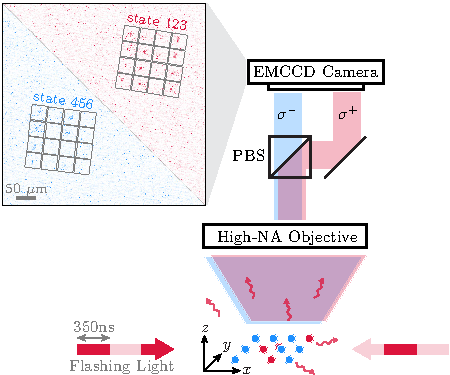
\includegraphics{fig-ai/spin-proc.pdf}
    \caption{
	\textbf{Spin-resolved fluorescence imaging setup.} 
	Atoms in states $\ket{3}$ (red) and $\ket{6}$ (blue) are illuminated by alternating flashing beams to suppress recoil-induced diffusion. Fluorescence photons emitted by the atoms are collected by a high-NA (0.65) objective, split by a polarizing beam splitter (PBS), and imaged onto distinct regions of an EMCCD camera, enabling single-shot spin resolution. Inset: representative fluorescence raw image.
	}
    \label{fig:spin-proc}
\end{figure}


\textbf{Free-space imaging.} Free-space fluorescence imaging represents an alternative approach to traditional Raman-cooled quantum gas microscopy, where atoms are imaged without confining potentials during the detection process. This paradigm eliminates the technical complexity of maintaining tight trapping and cooling during imaging, potentially enabling faster detection protocols and simplified experimental setups.

The Heidelberg group demonstrated pioneering work in spin-resolved free-space imaging of fermionic $^6$Li atoms \cite{bergschneider_spin-resolved_2018}. Their approach achieved single-atom detection fidelities of up to 99.4(3)\% by collecting approximately 20 fluorescence photons per atom during a 20 $\mu$s exposure. To mitigate acceleration from radiation pressure, they employed two counter-propagating laser beams with alternating 200 ns pulse sequences. Spin resolution was implemented through sequential imaging schemes, where different hyperfine states were addressed in successive exposures by shifting laser frequencies. While this sequential approach enabled spin-selective detection, it inherently limited access to simultaneous spin-spin correlations. Recent developments by the Greiner group have significantly advanced the speed and efficiency of free-space detection protocols \cite{su_fast_2025}. Their implementation achieved detection times as short as 2.4 $\mu$s while maintaining high detection fidelities. The demonstrated capability for parity-projection-free imaging represents a significant advantage, enabling direct counting of multiple atoms per site without light-assisted collisions.

For experiments requiring small lattice spacings, matter-wave magnification (MWM) has emerged as a crucial enabling technology \cite{murthy_matter-wave_2014, asteria_quantum_2021}. MWM techniques coherently expand atomic distributions before detection, circumventing diffraction-limited resolution while preserving site-resolved capability. By adiabatically manipulating harmonic potentials, spatial patterns can be magnified by factors of 10-50, enabling free-space imaging of systems with sub-micrometer lattice spacings.

The technical implementation of free-space imaging requires optimization of competing factors: imaging duration must be minimized to prevent significant atomic motion due to photon recoil, while collecting sufficient photons for reliable detection. For $^6$Li atoms, the relatively large recoil energy leads to position spreads of approximately 10 $\mu$m during typical imaging times. Performance trade-offs between free-space and lattice-based approaches depend on experimental priorities: free-space imaging offers superior detection speed, reduced complexity and simultaneous multi-component detection capabilities, while lattice-based methods typically provide better spatial resolution.


% \textbf{This work.} 
This work implements spin-resolved free-space imaging for $^6$Li atoms using simultaneous detection of stretched states $|3\rangle$ and $|6\rangle$ with polarization-selective optics. Atoms are transferred to these stretched states, which exhibit nearly pure $m_J = \pm 1/2$ character at high magnetic fields and couple strongly to $\sigma^{\pm}$ polarized light. A polarizing beam splitter after the imaging objective spatially separates the $\sigma^+$ and $\sigma^-$ fluorescence components onto distinct regions of the camera.

The implementation achieves 99\% spin discrimination fidelity while maintaining imaging times of 20 $\mu$s. Compared to previous approaches \cite{bergschneider_spin-resolved_2018}, which required sequential imaging cycles within a single experimental shot, our single-exposure detection simplifies the experimental sequence.
 % and reduces sensitivity to technical fluctuations. While the fundamental capabilities are similar, the streamlined approach facilitates integration with the rapid experimental cycles necessary for high-statistics studies of quantum dynamics.

The technique provides access to spin-dependent observables including local magnetization $\langle \sigma^z_i \rangle$ and spin correlations, essential for characterizing magnetic phenomena in Fermi-Hubbard systems. 
% The fast imaging protocol is designed for compatibility with the deterministic state preparation capabilities described in Section 4, enabling systematic studies of many-body dynamics with precisely controlled initial conditions.
Future integration with optical lattice system and MWM will enable
% transfer of deterministically prepared atomic configurations for 
investigation of dynamical phases including quantum thermalization, Anderson localization, and many-body localization. 
% Combined with the numerical simulation framework presented in Section 5, 
% This platform provides tools for systematic exploration of strongly correlated quantum matter in controllable fermionic systems.